\documentclass[12pt]{article}
\usepackage[utf8]{inputenc}
\usepackage{upquote}
\usepackage[margin=20mm]{geometry} 
\usepackage{amsmath,amsthm,amssymb}
\usepackage{graphicx}
\usepackage{listings}
\newenvironment{statement}[2][Statement]{\begin{trivlist}
\item[\hskip \labelsep {\bfseries #1}\hskip \labelsep {\bfseries #2.}]}{\end{trivlist}}
\usepackage{xcolor}
\usepackage{subfigure}


% Listings package for code rendering (No external dependencies)
\usepackage{listings}  
\usepackage{xcolor}   % Color support
\usepackage{tcolorbox} % Box for better appearance

% Define custom colors for code highlighting
\definecolor{codegreen}{rgb}{0,0.6,0}
\definecolor{codegray}{rgb}{0.5,0.5,0.5}
\definecolor{codepurple}{rgb}{0.58,0,0.82}
\definecolor{backcolour}{rgb}{0.95,0.95,0.92}


\lstset{frame=tb,
    language=Python,
    backgroundcolor=\color{backcolour},   
    commentstyle=\color{codegreen},
    keywordstyle=\color{magenta},
    numberstyle=\tiny\color{codegray},
    stringstyle=\color{codepurple},
    basicstyle=\ttfamily\footnotesize,
    breakatwhitespace=false,         
    breaklines=true,                 
    keepspaces=true,                 
    numbers=left,       
    numbersep=5pt,                  
    showspaces=false,                
    showstringspaces=false,
    showtabs=false,                  
    tabsize=2,
}




\title{Assignment 2}


%\author{Author \\
%  Wanjing Hu / fng685@alumni.ku.dk  \\
%  Shuangcheng Jia/   \\
%  Zhigao Yan / sxd343@alumni.ku.dk  \\
%} 
 

\begin{document}
\maketitle

\section{Pixel-wise contrast enhancement}
\subsection{Gray scale Image}
%wanjing
\begin{lstlisting}
def gamma_transform(image, gamma):
    # Normalize to [0,1]
    image = image.astype(np.float32) / 255.0 
    # Apply gamma correction
    corrected = np.power(image, gamma) 
    # Convert back to [0,255]
    return (corrected * 255).astype(np.uint8) 
\end{lstlisting}

A gamma=1 is equals to the original gray-scale picture, a gamma=0.5 makes dark regions look brighter, and a gamma=2.0 darkens bright regions. See figure~\ref{fig:1.1}.

\begin{figure}[ht]
\centering
    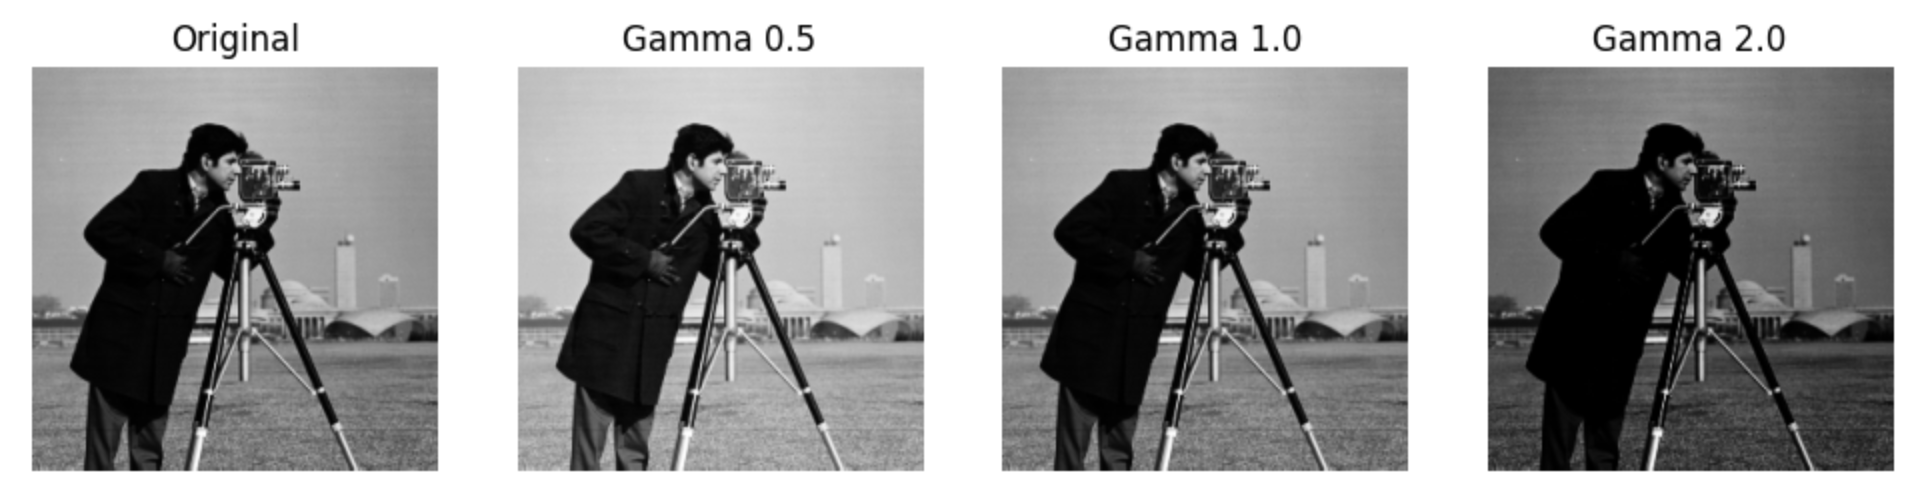
\includegraphics[width=0.7\columnwidth, keepaspectratio]{pics/a2-1.1}
\caption[]{Pixel-wise contrast enhancement on a gray scale picture}
\label{fig:1.1}
\end{figure}

\subsection{Color Image - RGB correction}

 See figure~\ref{fig:1.2}.

\begin{lstlisting}
def gamma_correct_hsv(image, gamma):
    hsv_image = color.rgb2hsv(image)
    hsv_image[..., 2] = 
      gamma_transform(
      	(hsv_image[..., 2] * 255).astype(np.uint8), gamma) / 255.0
    return (color.hsv2rgb(hsv_image) * 255).astype(np.uint8)
\end{lstlisting}
\begin{figure}[ht]
\centering
    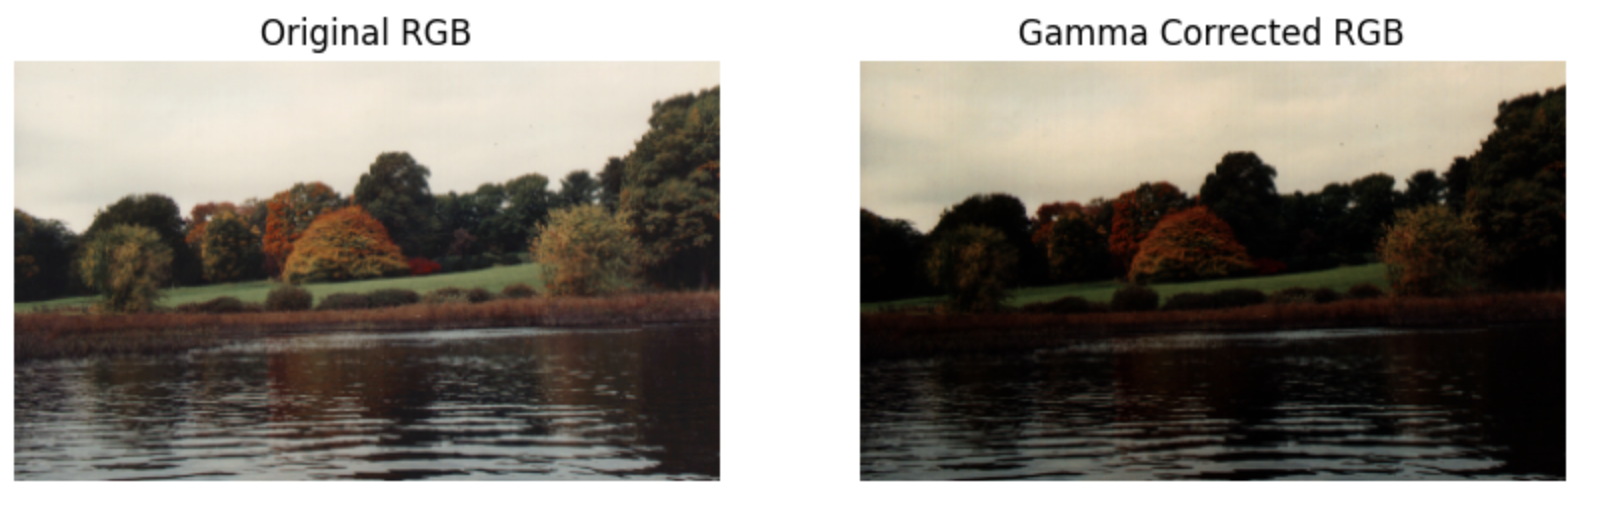
\includegraphics[width=0.7\columnwidth, keepaspectratio]{pics/a2-1.2}
\caption[]{Pixel-wise contrast enhancement on a gray scale picture}
\label{fig:1.2}
\end{figure}

\subsection{Color Image - HSV color representation}

\begin{lstlisting}
def gamma_correct_hsv(image, gamma):
    hsv_image = color.rgb2hsv(image)
    hsv_image[..., 2] = 
      gamma_transform((hsv_image[..., 2] * 255).astype(np.uint8), gamma) / 255.0
    return (color.hsv2rgb(hsv_image) * 255).astype(np.uint8)
\end{lstlisting}

 See figure~\ref{fig:1.3}. 
 The result of the RGB Correction is a little more brighter on the bright part, and thus look less natural. This may because the RGB Correction alters all channels independently, and the colors may be distorted. The HSV Correction modifies only the brightness while preserving colors, so it looks better.

\begin{figure}[ht]
\centering
    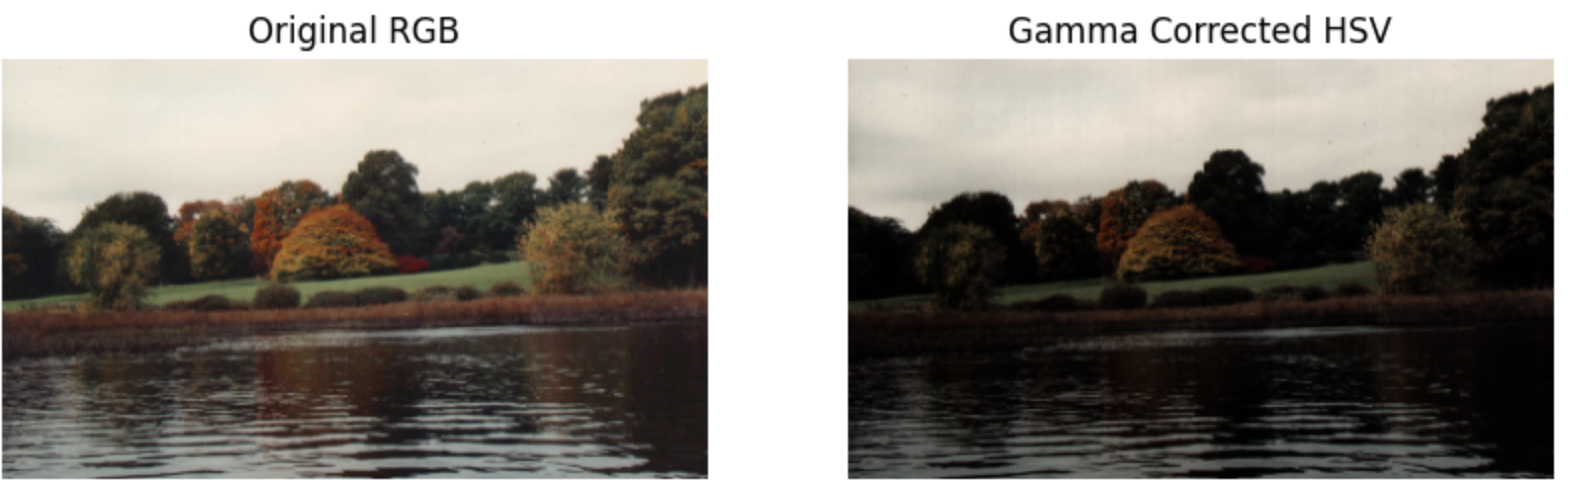
\includegraphics[width=0.7\columnwidth, keepaspectratio]{pics/a2-1.3}
\caption[]{Pixel-wise contrast enhancement on a gray scale picture}
\label{fig:1.3}
\end{figure}

\section{Reverb convolution}
%wanjing
\subsection{Plot laugh2.wav}
See figure ~\ref{fig:2.1}. The orange curve represents right sound track, and the blue curve represents the left sound track. The height of the curve represents the amplitude of this audio channel over time, with x-axis as time and y-axis as amplitude.
The sample rate represents how many samples per second are used to represent the sound.

\begin{figure}[ht]
\centering
    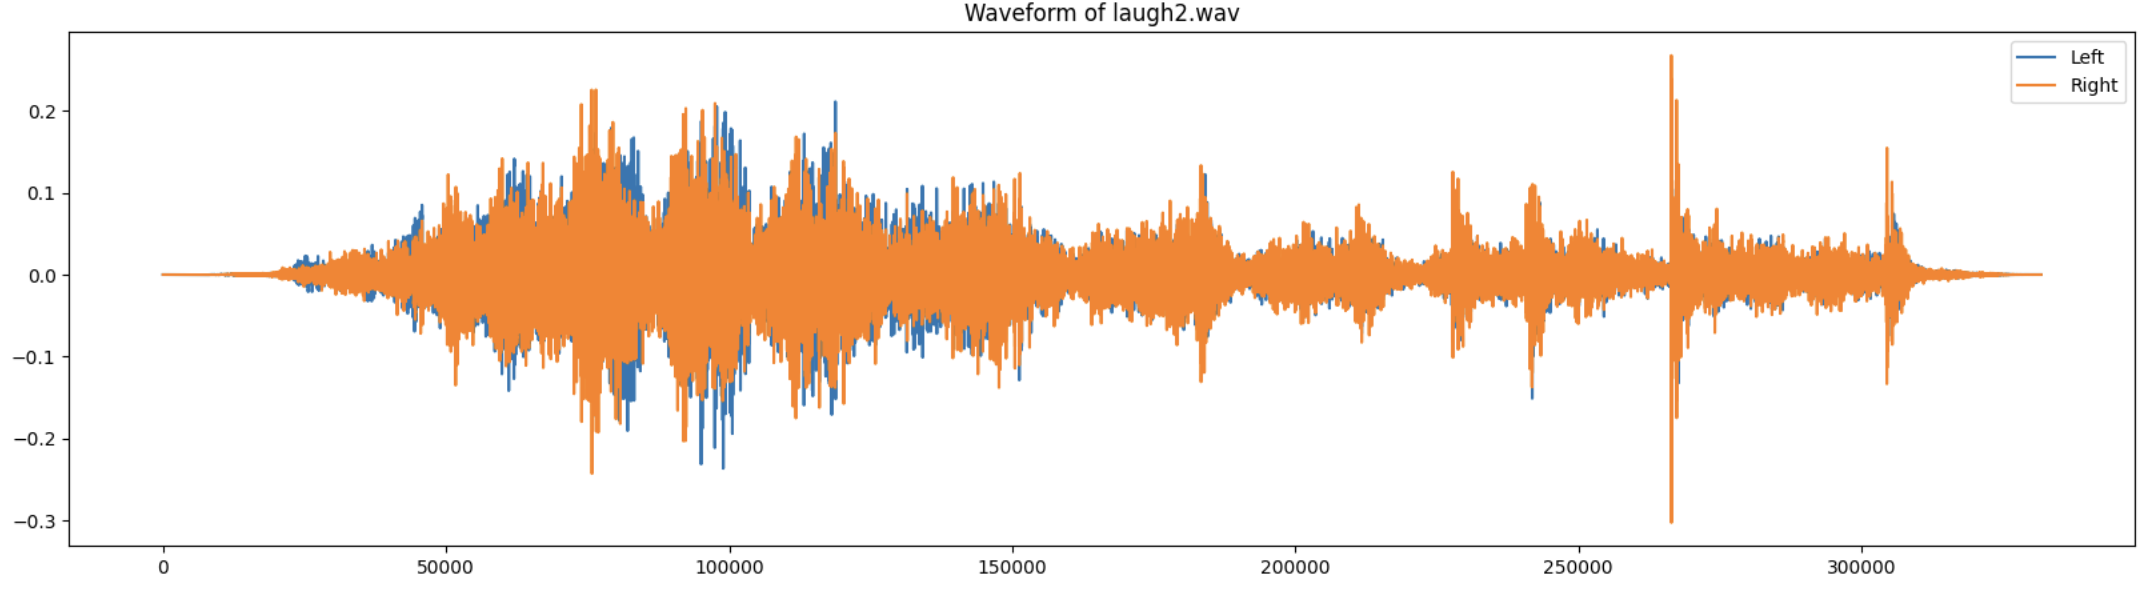
\includegraphics[width=0.7\columnwidth, keepaspectratio]{pics/a2-2.1}
\caption[]{Plot laugh2.wav}
\label{fig:2.1}
\end{figure}

\subsection{Reverb}

Reverb simulates sound reflections in space, making it feel more spacious and echoing.
With the convolution of Clap, the reverb mix the clap and the origin laughter, and it sounds like the laughter is mixed with claps in a hall. See ~\ref{ig:f2.1.2}.
With the convolution of Splash, the laughter sounds like coming from the outer space.  See ~\ref{ig:f2.1.3}.


\begin{figure}[ht]
\centering
\subfigure[Original Signal]{
    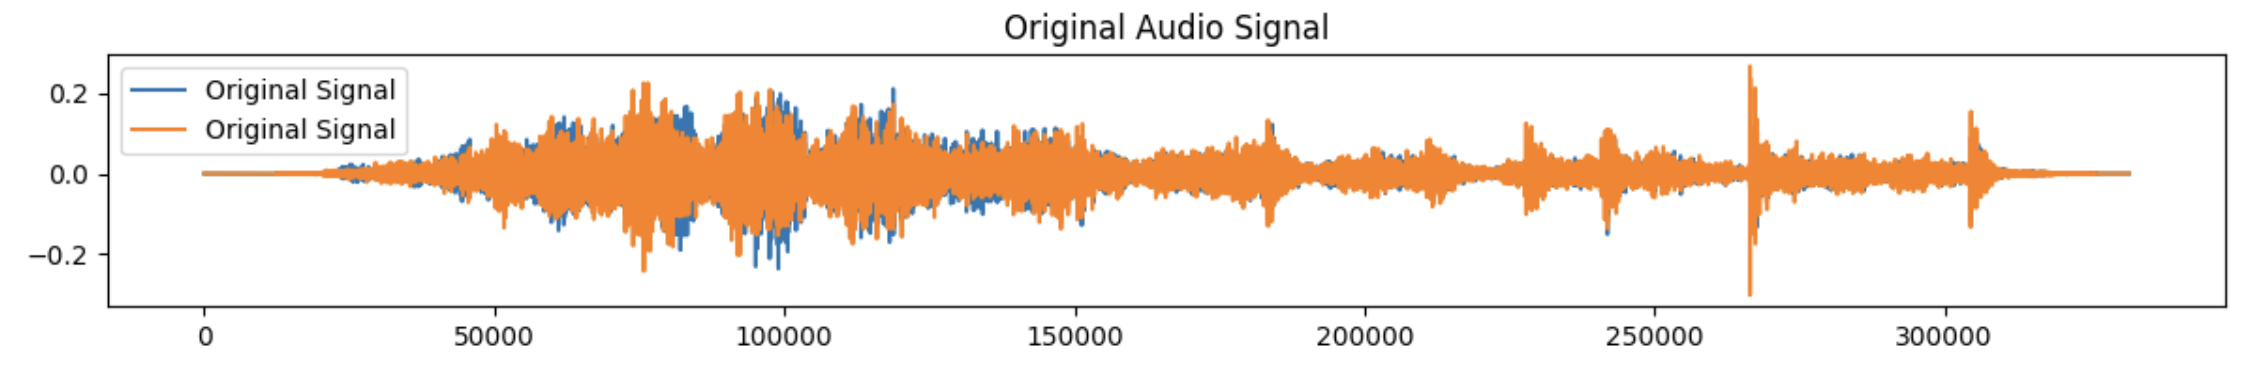
\includegraphics[width=0.7\columnwidth, keepaspectratio]{pics/a2-2.2-origin}
\label{fig:f2.1.1}
}
\subfigure[Response Signal, Clap]{
    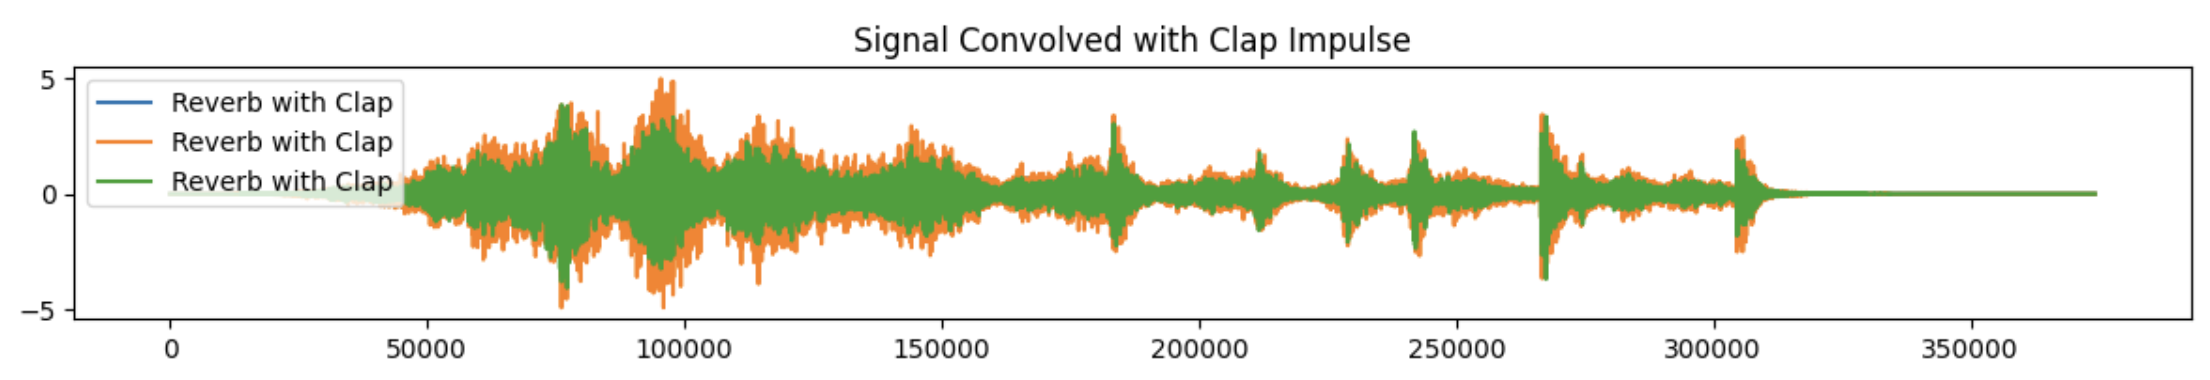
\includegraphics[width=0.7\columnwidth, keepaspectratio]{pics/a2-2.2-clap}
\label{fig:f2.1.2}
}
\subfigure[Response Signal, Splash]{
    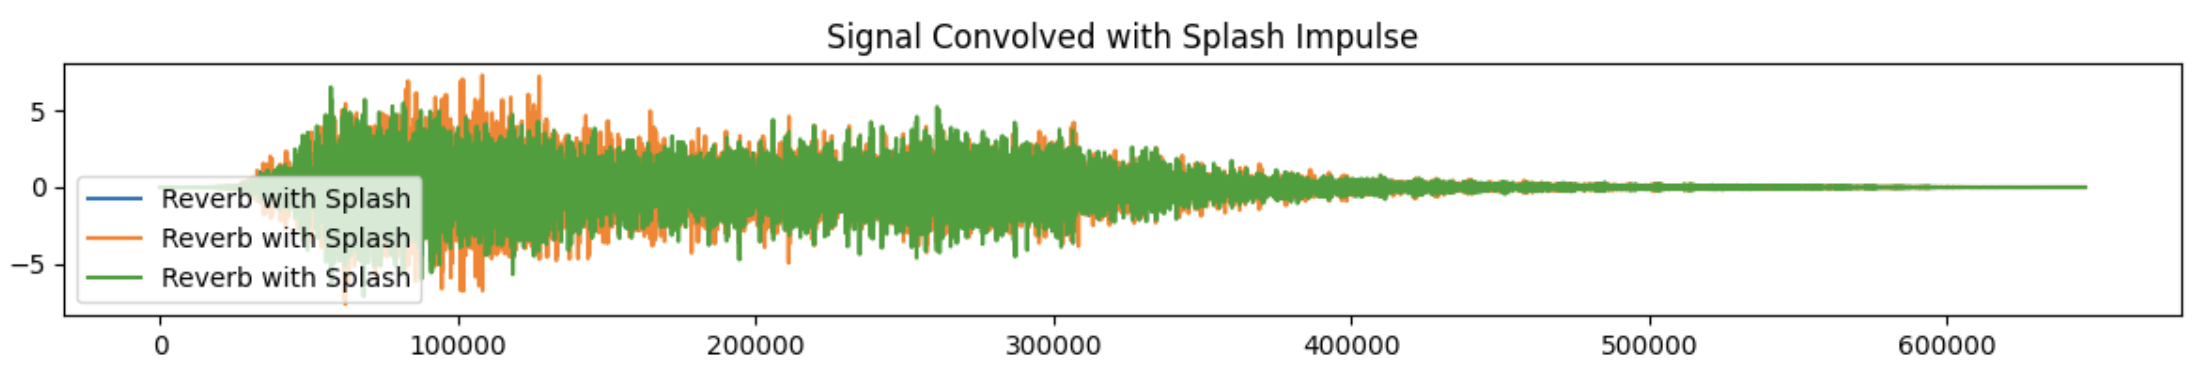
\includegraphics[width=0.7\columnwidth, keepaspectratio]{pics/a2-2.2-splash}
\label{ig:f2.1.3}
}

\caption[]{Plot laugh2.wav}
\label{fig:2.1}
\end{figure}

\subsection{Longer explanation}

The convolution operation matches the two inputs and do calculation. The output size is $len(signal)+len(impulse)-1$. In our case, the convolution blends the original waveform with the impulse response and adds tail reflections.

\section{Image filtering and enhancement}
%zhigao

\section{Histogram-based processing}
%shuangcheng


\end{document}
